%%%%%%INTRODUZIONE
\chapter{Angular, libreria e funzionalità}
\section{Introduzione alla tecnologia}
Angular è una libreria per lo sviluppo di interfacce web di tipologia s.p.a. (single page application) con paradigma a componenti strutturata per lo sviluppo di software ad alta manutenibilità e prestazioni.

Offre diverse funzionalità tra cui:
\begin{itemize}
    \item Sviluppo a componenti concepiti come singoli elementi di visualizzazione dei dati
    \item Dependency injection
    \item Possibilità di strutturazione dei componenti in raggruppamenti chiamati moduli
    \item Gestione degli eventi e possibilità di generazione degli stessi
    \item Routing tra i componenti che compongono la web-app
    \item Rendering dei componenti del DOM a runtime con monitoraggio delle variazioni e conseguente aggiornamento tramite change detection
\end{itemize}
Le applicazioni Angular sono composte da un insieme di componenti organizzati in moduli che vengono renderizzati in una struttura ad albero, i componenti possono condividere dati tramite le properties e gli eventi.
\newline
\newline
La dependency injection è realizzata tramite i service, classi typescript istanziate dal framework il cui scopo è fornire ai componenti la logica applicativa complessa necessaria al loro funzionamento.
\newline
\newline
I componenti e i service sono raggruppati in moduli i quali fungono da elemento organizzativo dell'applicazione, i moduli stessi possono importare ed esportare componenti e servizi.
\newline
\newline
Il framework consente di effettuare il routing fra i vari componenti dell'applicazione che vengono renderizzati all'interno del DOM, in questo modo è possibile far variare i componenti visualizzati a schermo in base all iterazione con l'utente.
\newline
\newline
Tramite il meccanismo di Change detection, la libreria Angular è in grado di rilevare le modifiche effettuate alle proprietà dei componenti e aggiornare il DOM di conseguenza.
\newline
\newline
La libreria è distribuita come modulo Node.js e sfrutta npm (node packet manager) per la gestione delle dipendenze e l'istallazione di librerie di componenti angular aggiuntivi come per esempio la libreria di componenti nebular.
\newline
\newpage%%% COMPONENTI STRUTTURA
\section{Componenti Angular}
I componenti rappresentano l'elemento base di un'applicazione Angular e sono composti da 3 elementi principali:
\begin{itemize}
    \item Una classe Typescript che ne implementa il comportamento e le proprietà
    \item Un template HTML che ne definisce la vista renderizzata all'interno del DOM
    \item Un file css che ne definisce lo stile
\end{itemize}
Il comportamento dei componenti viene fornito da una direttiva Component che fornisce i metadati necessari alla creazione gestione e eliminazione del componente tra cui:
\begin{itemize}
    \item Il CSS selector
    \item Il template del componente
    \item Il foglio di stile
    \item I provider degli eventuali servizi di cui il componente potrà usufruire
\end{itemize}
In particolare è proprio il @Component decorator che identifica la classe Typescript come componente alla libreria angular, il quale senza non viene riconosciuto come tale.
\newline
Una parte fondamentale di ogni componente è il CSS selector che è il nome con cui viene riconosciuto dalla libreria e indica di renderizzare il componente ogni qualvolta viene trovato il corrispettivo tag.
\newline
\subsection{Angular template}
Il template definisce ciò che viene renderizzato nel DOM all'istanziazione,
al suo interno è possibile sfruttare il data binding dei componenti  per referenziare le proprietà definite nella classe typescript e sfruttare le direttive Angular per rendere dinamica la costruzione del DOM.
\newline
\newline
\begin{figure}[H]
    \centering
    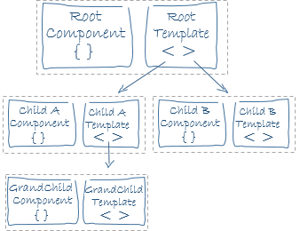
\includegraphics[scale=1]{resources/component-tree.png}
    \cite{angular-doc}
    \caption{struttura albero dei componenti}
\end{figure}

Il template di un componente e la sua classe typescript formano una view, la quale può includere altre view al suo interno in una struttura gerarchica ad albero.
\newline
Il template di un componente angular è scritto in codice HTML esteso dalla sintassi Angular per il template, la quale si occupa di alterare il DOM a seconda della logica applicativa e della variazione dei dati.
Come già anticipato, all'interno del template è possibile sfruttare:
\begin{itemize}
    \item Direttive per applicare logica al rendering del component (ngFor)
    \item Pipe per trasformare i dati prima di mostrarli a schermo
    \item Data binding tra proprietà della classe e template
\end{itemize}
Le direttive sono classi typescript contenenti il decorator @directive che consentono di rendere il template dei componenti dinamico e si suddividono in due tipologie:
\begin{itemize}
    \item Direttive strutturali
    \item Direttive attributo
\end{itemize}
Le direttive strutturali alterano il DOM aggiungendo rimuovendo o modificando elementi come le direttive ngFor e ngIf,
mentre le direttive attributo alterano il DOM modificando il valore di singoli attributi.
\newline
\newline
Le pipe sono strumenti attraverso i quali è possibile manipolare i dati da mostrare nel DOM tramite particolari sequenze di istruzioni come per esempio la formattazione di dati nel formato locale dell'utente oppure la formattazione di valute.
\newline
\newline
Una delle operazioni più tediose e inclini alla generazione di errori nelle interfacce web è la necessità di collegare i dati mostrati all'interno dell'interfaccia con ciò che viene manipolato dalla logica applicativa. Tramite il data binding la libreria Angular automatizza questo processo come mostrato nell'immagine sottostante
\newline
\newline
\begin{figure}[H]
    \centering
    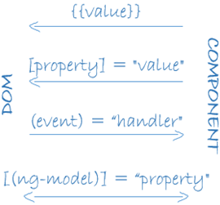
\includegraphics[scale=1]{resources/databinding.png}
    \cite{angular-doc}
    \caption{Modalità di funzionamento data binding}
\end{figure}
nell'immagine viene mostrata la possibilità di implementazione del data binding in 3 possibili modalità:
\begin{itemize}
    \item Monodirezionale dal component al dom
    \item Monodirezionale dal dom al component
    \item Bidirezionale
\end{itemize}
In questo modo viene automatizzata una procedura molto onerosa e che molto spesso rende illeggibili le interfacce di molte applicazioni web%%%%%%% CICLO DI VITA COMPONENTI
\section{Ciclo di vita dei componenti}
I componenti Angular seguono il seguente lifecicle:

\begin{itemize}
    \item Istanziazione del componente e renderizzazione dello stesso e dei componenti figli all'interno del DOM
    \item Aggiornamento del componente secondo la strategia di aggiornamento al cambio delle proprietà dello stesso
    \item Distruzione del componente e dei rispettivi componenti e conseguente rimozione del componente dal DOM
\end{itemize}

È possibile definire comportamento aggiuntivo del componente ad ognuna delle fasi del ciclo di vita implementando i rispettivi metodi definiti dalla direttiva Component.
I metodi sono i seguenti:

\begin{itemize}
    \item ngOnInit() si occupa del rendering nel DOM del componente, chiamato una volta sola alla renderizzazione  del componente
    \item ngOnChanges() si occupa di aggiornare il componente quando la libreria modifica almeno una delle proprietà del componente
    \item ngOnDestroy() chiamato subito prima della distruzione di un componente
    \item ngDoCheck() per dare la possibilità di rilevare modifiche alle proprietà dei componenti che la libreria non rileva viene reso disponibile il metodo ngDoCheck() che permette di implementare la strategia di rendering desiderata
\end{itemize}

Le chiamate ai metodi ngOnChanges() e ngDoCheck() se definiti avvengono molto di frequente nella vita di un componente portando a importanti cali di prestazioni in caso di implementazioni esose dei metodi. In particolare, il metodo ngDoCheck() viene chiamato con estrema frequenza a ogni ciclo di scansione del DOM, anche se il componente non ha subito cambiamenti.
\begin{figure}[H]
    \centering
 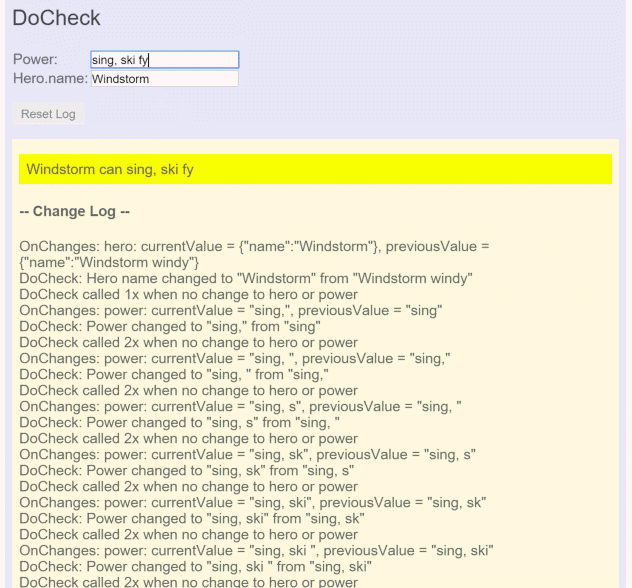
\includegraphics[scale=0.5]{resources/doCheck.png}
 \cite{angular-doc}
    \caption{funzionamento metodo ngDocheck()}
\end{figure}
come si può vedere nell'esempio, il metodo  ngDoCHeck viene chiamato diverse decine di volte anche se non avviene nessuna variazione ai valori dei due campi input.
\newline
Il metodo ngOnInit() è fondamentale nel caso di fetch di dati da un servizio remoto, essendo chiamato alla visualizzazione del componente consente di ritardare il fetch dei dati al momento in cui ce n'è un vero bisogno ed evitare il costoso fetch dei dati da parte del costruttore che rallenterebbe di molto i tempi di load dell'applicazione.
\newline
\newline
Il metodo NgOnDestroy() risulta utile per evitare memory leaks rimuovendo il componente da eventuali emettitori di eventi.
%%%%%%%%%%MODULI
\section{Organizzazione dei componenti, i Moduli}
Uno dei concetti principali del framework Angular è il rendere le applicazioni il più modulari possibile. Per realizzarla la libreria propone il concetto di ngModule, un ngModule consiste in un raggruppamento di entità angular dedicate all'implementazione di una particolare sotto funzionalità, un servizio necessario all'applicazione o un particolare step dell'applicazione.
Un ngModule può contenere al suo interno:
\begin{itemize}
    \item Componenti
    \item Service
    \item Qualunque altro file utile allo sviluppo della funzionalità offerta dal modulo
\end{itemize}
Ogni applicazione Angular è formata da un insieme di ngModule dei quali ne è sempre presente uno radice (root) il quale viene lanciato all'avvio dell'applicazione.
Cosi come i componenti, anche gli ngModule sono organizzati in una struttura ad albero,
della quale la radice è l' ngModule root
\subsection{Metadati}
un ngModule è definito da una classe typescript con decorator @ngModule il quale definisce i suoi metadati:
\begin{itemize}
    \item La lista di componenti direttive e service che fanno parte del ngModule
    \item Gli elementi che sono visibili e utilizzabili dagli altri moduli
    \item Gli elementi che sono importati da altri moduli
    \item Tutti i fornitori di service che questo modulo espone all'esterno
    \item Il componente root del modulo
\end{itemize}
Ogni ngModule crea un ambiente di compilazione isolato per le entità al suo interno e possiede un componente root che viene caricato al boot, ma è comunque possibile accedere agli altri componenti del ngModule tramite il routing o il rendering del template del singolo componente
\begin{figure}[H]
    \centering
   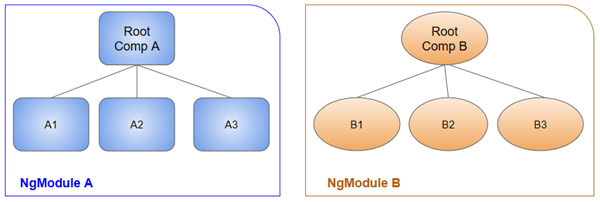
\includegraphics[scale=1]{resources/compilation-context.png}
   \cite{angular-doc}
    \caption{rappresentazione ambiente di compilazione dei moduli}
\end{figure}


come mostrato nell'immagine i due ngModule offrono ambienti di compilazione differenti per i moduli all'interno, questo consente alle applicazioni angular di essere pienamente modulari dato che i singoli moduli sono pienamente indipendenti.
\newline
Come mostrato dall'immagine sottostante, le view possono essere organizzate in gerarchie, che rappresentano singole aree di visualizzazione all'interno della pagina,esse vengono gestite dalla libreria come una unica entità e possono contenere componenti da ngModule differenti
\begin{figure}[H]
    \centering
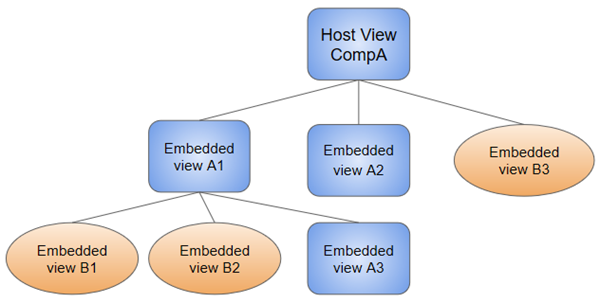
\includegraphics[scale=1]{resources/view-hierarchy.png}
   \cite{angular-doc}
    \caption{rappresentazione gerarchia delle view}
\end{figure}
\newpage
\section{ Implementazione della dependency injection, i Services}
I componenti angular idealmente dovrebbero occuparsi esclusivamente di rendere possibile la user experience costruendo la vista applicativa e sfruttando il data binding per gestire la logica applicativa.
\newline
Per tutti i compiti esterni alla logica applicativa, Angular propone il concetto di Service.
\newline
I Service sono classi typescript descritte dal decorator @Injectable il cui compito è quello di occuparsi delle operazioni di utilità necessarie al funzionamento dei componenti.
Le operazioni gestite dai service possono includere:
\begin{itemize}
    \item Fetch dei dati da datasource esterne
    \item Logging delle operazioni o di debug
    \item Validazione del input utente
\end{itemize}
Grazie ai service è possibile rendere i componenti indipendenti da queste operazioni e rendere riusabile la struttura della vista utente.
In questo modo i componenti non sono vincolati a particolari sistemi esterni, (ad esempio datasource) che possono avere concezioni di immagazzinamento dei dati differenti.

\subsection{Dependency Injection}
La dependency injection è una funzionalità diventata ormai fondamentale nelle applicazioni enterprise di grandi dimensioni, sia per testing del sistema sia per aumentare la riusabilità e la modularità delle applicazioni. Essa permette di rovesciare la logica di ottenimento delle dipendenze di un particolare componente sofware, liberando il componente dall'obbligo di reperire le dipendenze e delegando a altre entità il compito.
\begin{figure}[H]
    \centering
 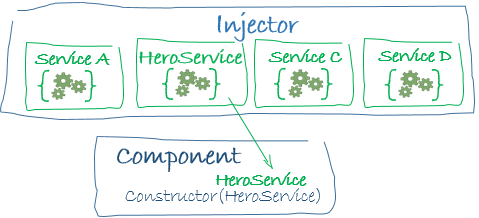
\includegraphics[scale=0.75]{resources/injector-injects.png}
\cite{angular-doc}
   \caption{rappresentazione oggetto Injector}
\end{figure}
La libreria Angular implementa questa funzionalità attraverso i service, essi possono essere richiesti dal costruttore di un componente e vengono forniti dal framework alla creazione dello stesso tramite un oggetto chiamato Injector, in questo modo il componente necessita solo di dichiarare il service di cui ha bisogno e non di definirne la logica di funzionamento o di occuparsi della sua creazione o istanziazione.
\newline
\newline
Un service, per poter essere iniettato all'interno di un componente necessita un provider che consente di definire la visibilità del service.
Quest'ultima può essere:
\begin{itemize}
    \item A livello di componente, in questo caso per ogni istanza dello specifico componente viene creata un istanza del service
    \item A livello di ngModule, in questo modo viene creata una sola istanza per tutti i componenti che fanno parte di quel service
    \item A livello radice, in questa modalità viene creata una sola istanza del service, che viene resa disponibile a tutti i componenti interni all'applicazione
\end{itemize}
La capacità dei provider di limitare la visibilità dei service è fondamentale anche sotto un punto di vista di ottimizzazione delle prestazioni, in quanto consente di istanziare i service solo in caso si utilizzi il componente applicativo che ne ha un effettivo bisogno.
\newpage
\section{Routing dei componenti Angular}
Una delle funzionalità fondamentali per una single page application è la possibilità di navigare tra le varie viste senza interrogare il server per reperire una nuova pagina.
La libreria Angular consente di navigare tra le viste del' applicazione tramite il package routing, distribuito esternamente rispetto al core.
\newline
\newline
La libreria implementa la funzionalità tramite l'oggetto routing, gestito tramite il pattern singleton e creato all'avvio dell'applicazione, l'oggetto è in grado di tradurre gli url in componenti da renderizzare all'interno della pagina.
Le associazioni tra url e componenti vengono effettuate all'interno della definizione del ngModule, tramite il metodo
\begin{lstlisting}{javascript}
    RouterModule.forRoot();
\end{lstlisting}
al quale viene fornito, come argomento, un array contenete le coppie url componente.
La renderizzazione dell'output del routing angular avviene all'interno della direttiva
\begin{lstlisting}{html}
    <router-outlet></router-outlet>
\end{lstlisting}
Alla fine di ogni ciclo di navigazione, la libreria costruisce un albero per rappresentare lo stato corrente del router, disponibile a tutti i componenti tramite il service Router.
\newpage\section{Gestione runtime dei componenti, il meccanismo change detection}
Per consentire l'aggiornamento runtime  del DOM a seguito delle modifiche delle proprietà dei componenti, Angular sfrutta un meccanismo chiamato change detection.
\newline
 La libreria costruisce un albero composto dai componenti renderizzati e, quando viene lanciato il meccanismo di change detection, essa esegue una visita top down dell'albero in cerca dei componenti le quali proprietà sono state modificate e ne renderizza di nuovo la view. Angular esegue questa operazione solo per le proprietà che vengono utilizzate nel template e per ognuna esegue un controllo con il valore precedente.
\newline
\begin{figure}[H]
\centering
   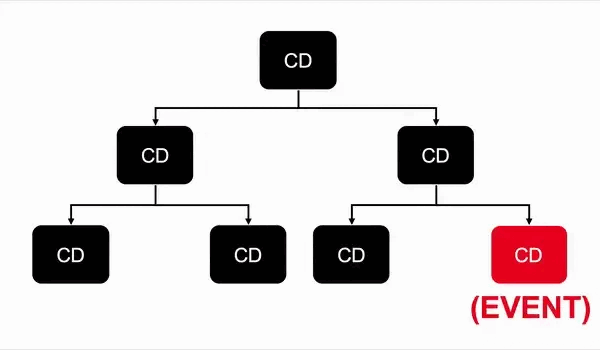
\includegraphics[scale=0.5]{resources/cd-1.png}
\caption{un componente viene modificato e lancia il meccanismo di change detection}
\end{figure}
\begin{figure}[H]
\centering
   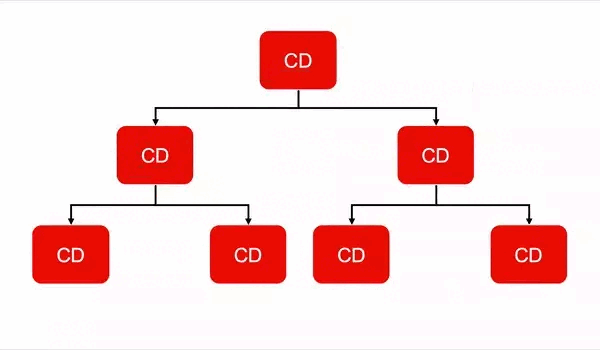
\includegraphics[scale=0.5]{resources/cd-2.png}
\caption{l'albero viene visitato alla ricerca di proprietà modificate}
\end{figure}





\section{Change detection: innesco del meccanismo}

Per poter consentire il corretto avvio del meccanismo la libreria angular modifica il comportamento standard di alcuni metodi di basso livello del motore javascript:
\begin{itemize}
    \item Tutti gli eventi del browser (click, mouseover, keyup, etc. )
    \item Le chiamate ajax HTTP
    \item I metodi setTimeout() e setInterval()
\end{itemize}
Angular inoltre si avvale della libreria zone.js per modificare in maniera trasparente i comportamenti del browser e innescare il meccanismo di change detection come mostrato nell'esempio.
\newline
\begin{lstlisting}{javascript}
        // this is the new version of addEventListener
function addEventListener(eventName, callback) {
     // call the real addEventListener
     callRealAddEventListener(eventName, function() {
        // first call the original callback
        callback(...);
        // and then run Angular-specific functionality
        var changed = angular.runChangeDetection();
         if (changed) {
             angular.reRenderUIPart();
         }
     });
}

\end{lstlisting}
\cite{angular-doc}

\section{Cange detection: strategie}
Il meccanismo di change detection può avvenire in due principali strategie
\begin{itemize}
    \item Default
    \item OnPush
\end{itemize}
La libreria angular adotta la modalità default, che lancia il meccanismo di change detection ogni volta che viene lanciato un evento di interazione con l'utente, questo può portare a cali di prestazione soprattutto con alberi di componenti molto vasti.
È possibile modificare la strategia di change detection utilizzata all'interno della diretiva Compontent
\begin{lstlisting}{typescript}
    @Component({    selector: 'hero-card',
    changeDetection: ChangeDetectionStrategy.OnPush,
    template: ...
    })
    export class HeroCard {    ...}
\end{lstlisting}
I componenti che sfruttano la strategia onPush vengono aggiornati solo nei seguenti casi
\begin{itemize}
    \item Vengono modificati i riferimenti delle proprietà utilizzate nel template
    \item Viene lanciato un evento dal componente o da uno dei suoi figli
    \item Un oggetto osservabile collegato al template emette un nuovo evento
    \item La change detection viene attivata manualmente
\end{itemize}

\begin{figure}[H]
    \centering
 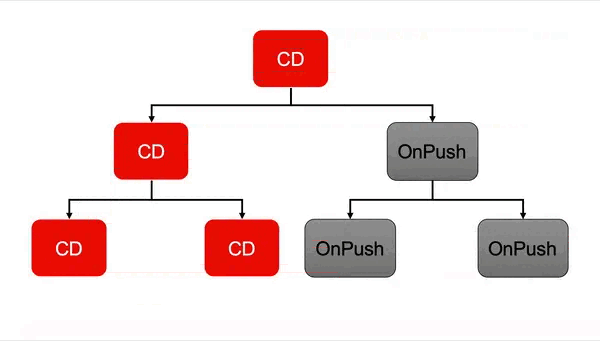
\includegraphics[scale=0.75]{resources/cd-onPush.png}
   \caption{Ciclo di change detection con componenti che sfruttano la strategia onPush}
\end{figure}
In questo modo è possibile evitare che il meccanismo di change detection venga eseguito su componenti di cui non è necessario effettuare sempre l'aggiornamento e rendere l'applicazione più responsiva.
\newline
La strategia onPush tuttavia prevede alcune accortezze per essere utilizzata correttamente. Per come è strutturata la strategia è necessario fornire al template una nuova istanza delle proprietà per poter attivare il meccanismo invece di modificare i valori associati alle proprieta.
\newline
Tuttavia gli oggetti javascript nascono come oggetti mutabili, questo comportamento del linguaggio facilita il manifestarsi di comportamenti non voluti da parte del meccanismo di Change dectection, è consigliabile quindi utilizzare librerie javascript che forniscano oggetti immutabili, come per esempio Immutable.js
